%% The following is a directive for TeXShop to indicate the main file
%%!TEX root = diss.tex

\chapter{Model of 3D Reconstruction}
\label{ch:3DRecon_Model}
In Chapter~\ref{ch:3DRecon_Taxo}, we introduce a taxonomy of 3D reconstruction which map algorithms according to the main visual cues used for reconstruction. In this chapter, we attempt to extend this mapping by providing a model of 3D reconstruction which allows for a well defined specification of the visual cues surrounding the problem and of the range of the desired solution, abstracting away from the functional specification of \textit{how} to estimate a reconstruction.

The goal when providing an abstraction to 3D reconstruction is that with better description should lead to better result. To order to achieve this, the visual and geometric properties of an object that can affect the visual cues should be examined in depth so that important aspects of the problem can be described.

A key requirement of the 3D reconstruction model is that it should be interpretable. Thus the components of this model must be well defined. We first propose a formal definition of the 3D reconstruction problem in Section~\ref{sec:3DRecon_Def}. Section~\ref{sec:3DRecon_Rep} explores the inputs and outputs used in 3D reconstruction problems. Section~\ref{sec:3DRecon_Desc} discusses various \textit{properties} that can be used to describe the appearance of the object. Section~\ref{sec:3DRecon_Exp} provides the mapping of the representations and properties into a formal model via which 3D reconstruction problem can be expressed. These layers: Definition, Representation, Conditions, and Expression represent out framework of accessible 3D reconstruction.

\section{Definition}
\label{sec:3DRecon_Def}
We first give the definition of some basic concepts, which encompass general computer vision concepts such as scene, camera, and image. We then define some other notions that are close related to the reconstruction problem before a formal definition is introduced. We then provide some reasonable approximations for a more practical definition.

\subsection{Basic notations}
We use the following notations: $\{C_n\}_{n=0}^{N-1}$ represents the camera set, which include both the intrinsic and extrinsic parameters; $\{L_n\}_{n=0}^{N-1}$ represents the set of light sources; and $\{I_n\}_{n=0}^{N-1}$ represents the set of all images.

\textbf{Definition 1 (Scene)} The scene $S$ is the four-dimensional joint spatio-temporal target of interest.

\textbf{Definition 2 (Image)} The transformation of the scene $S$ onto the image plane of camera $C_i$ at time $t_0$, which can be modelled as: $I_i = T(S, C_i, L_0, t_0)$, or the transformation of the scene $S$ onto the image plane of $C_0$  under the light source $L_i$ at time $t_i$, $I_i= T(S, C_0, L_i, t_i)$, where $T$ is the transformation.

The transformation can be a perspective projection which determines the 2D coordinates from a depth, or the BRDF function which determines the intensity/irradiance information from the information of illumination, viewing direction and surface orientation.

\subsection{Segment and Scelement}
Segments are the lowest level component we actively work with.

\textbf{Definition 3 (Segment)} A segment is a distinct region in the image, can be thought of as a generalization of pixel.

For instance, a segment can be a pixel, a window area, an edge, a contour, or a region of arbitrary size and shape.

\textbf{Definition 4 (Cue)} cues are the visual or geometric characteristics of the segments $seg$ that can be used for reconstruction, denoted as $cue(seg)$.

For instance, the cue can be texture within a window area, intensity/colour value of a pixel, or object contour, etc.

\textbf{Definition (Scelement)} A Scelement (scene element) is a distinct volume in the scene which corresponds to at least one segment, can be thought of as a generalization of a voxel.

\textbf{Definition (Scelement property)} Properties are the visual and geometric characteristics of the scelement $slmt$, which would influence the cues of a segment, denoted as $prop(slmt)$.

The property of the scelment can be the visual texture, diffuse albedo, surface orientation, roughness, convacity, etc.

\textbf{Definition (Scelement representation)} The scelement can be represented by voxels, depth, 3D coordinates, or surface orientation, etc, which is denoted as $rep(slmt)$.

\subsection{Photo-consistency}
Every photograph of a 3D scene taken from a camera $C_i$ partitions the set of all possible shape-radiance scene descriptions into two families, those that reproduce the photograph and those that do not. We characterize this constraint for a given shape and a given radiance assignment by the notion of \textit{photo-consistency}.

\textbf{Definition (Photo-consistency check)} The property of a scelement can produce the cue of the corresponding segment. $consist(rep(slmt), prop(slmt), cue(seg)).$
\begin{align*}
consist(rep(slmt), prop(slmt), cue(seg)) = 1 &\Rightarrow \textit{photo consistent}\\
consist(rep(slmt), prop(slmt), cue(seg)) = 0 &\Rightarrow \textit{not photo consistent}
\end{align*}
where $seg$ is the corresponding segment of scelement $slmt$.

\textbf{Definition (Segment photo-consistency)} Let $S$ be an arbitrary subset of $\mathbb{R}^3$. A scelement $p\in S$ that is visible from $C_i$ is photo-consistent with the image $I_i$ if and only if the photo-consistency check is true.

\textbf{Definition (Shape photo-consistency)} A scene $S$ is photo-consistent with image $I_i$ if all scelements visible from the camera $C_i$ are segment photo-consistent.

\textbf{Definition (Scene photo-consistency)} A scene $S$ is photo-consistent with a set of images $\{I_n\}_{n=0}^{N-1}$ if it's shape photo-consistency with each image in the set.

\subsection{Formal Definition}
\textbf{Definition (3D reconstruction)} Given a set of images $\{I_n\}_{n=0}^{N-1}$ captured by cameras $\{C_n\}_{n=0}^{N-1}$, or under a set of light sources $\{L_n\}_{n=0}^{N-1}$, find a set of scelements $\{slmt_n\}_{n=0}^{M-1}$ such that any scelement is photo-consistent with the image set $\{I_n\}_{n=0}^{N-1}$, \ie $\forall slmt_i\in \{slmt_n\}_{n=0}^{M-1}$, we have $consist(rep(slmt_i), prop(slmt_i), cue(seg_{(i, n)})) = 1$.

where $seg_{(i, n)}$ is the corresponding segment of $slmt_i$ in camera $C_n$. Alternatively, 3D reconstruction tries to find a set of scelments $\{slmt_n\}_{n=0}^{M-1}$ that are scene photo-consistent with the image set $\{I_n\}_{n=0}^{N-1}$

\subsection{Applied Definition}
While the definition presented above gives an definitive definition of the problem of 3D reconstruction, it does so in a purely theoretical way which is not necessarily applicable in a practical setting. We extend in this section this formal definition to an approximate, but more applied version.

\subsection{Applied photo-consistency}
\textbf{Definition (Photo-consistency check)} The property of a scelement can produce the cue of the corresponding segment. $consist(rep(slmt), prop(slmt), cue(seg))$.
\begin{align*}
consist(rep(slmt), prop(slmt), cue(seg)) = x
\end{align*}
where $x\in[0, 1]$, is a measure of similarity between the scelement and the corresponding segment, and
\begin{align*}
consist(rep(slmt), prop(slmt), cue(seg)) = 1 &\Rightarrow \textit{photo consistent}\\
consist(rep(slmt), prop(slmt), cue(seg)) = 0 &\Rightarrow \textit{not photo consistent}
\end{align*}

\subsection{Definition (Applied 3D Reconstruction)} Given a set of images $\{I_n\}_{n=0}^{N-1}$ captured by cameras $\{C_n\}_{n=0}^{N-1}$, or under a set of light sources $\{L_n\}_{n=0}^{N-1}$, find a set of scelements $\{slmt_n\}_{n=0}^{M-1}$ such that the photo-consistency measure between the set of scelements and their corresponding segments are maximized.

$$\mbox{maximize} \quad \sum_{n=0}^{N-1}\sum_{slmt_i\in \{slmt_j\}_{j=0}^{M-1}} consist(rep(slmt_i), prop(slmt_i), cue(seg_{(i, n)}))$$

where $seg_{(i, n)}$ is the corresponding segment of scelement $slmt_i$ in camera $C_n$.

\section{Representation}
\label{sec:3DRecon_Rep}
Based on the proposed definitions of 3D reconstruction problem, we need to further define the representations so that any developers can express their problem based on our proposed model. We look at the \textit{cues} that are utilized by 3D reconstruction techniques and their corresponding contributing properties. In Chapter~\ref{ch:3DRecon_Taxo}, we explored a new taxonomy of 3D reconstruction based visual/geometric cues. Now we need to investigate the visual and geometric properties of the object that can affect those cues. This section is organized by the visual/geomtric cues, and the visual/geomtric properties are investigated in each section.

\subsection{Texture}
\subsubsection{Segment and Scelement rerepsentation}
The segment is mostly a window area of pixels with varying window size. The scelement is typically a 3D point represented by a depth value along a line of sight, 3D coordinates, or a surface patch parametrized by depth and orientation.
\begin{figure}[h]
\centering
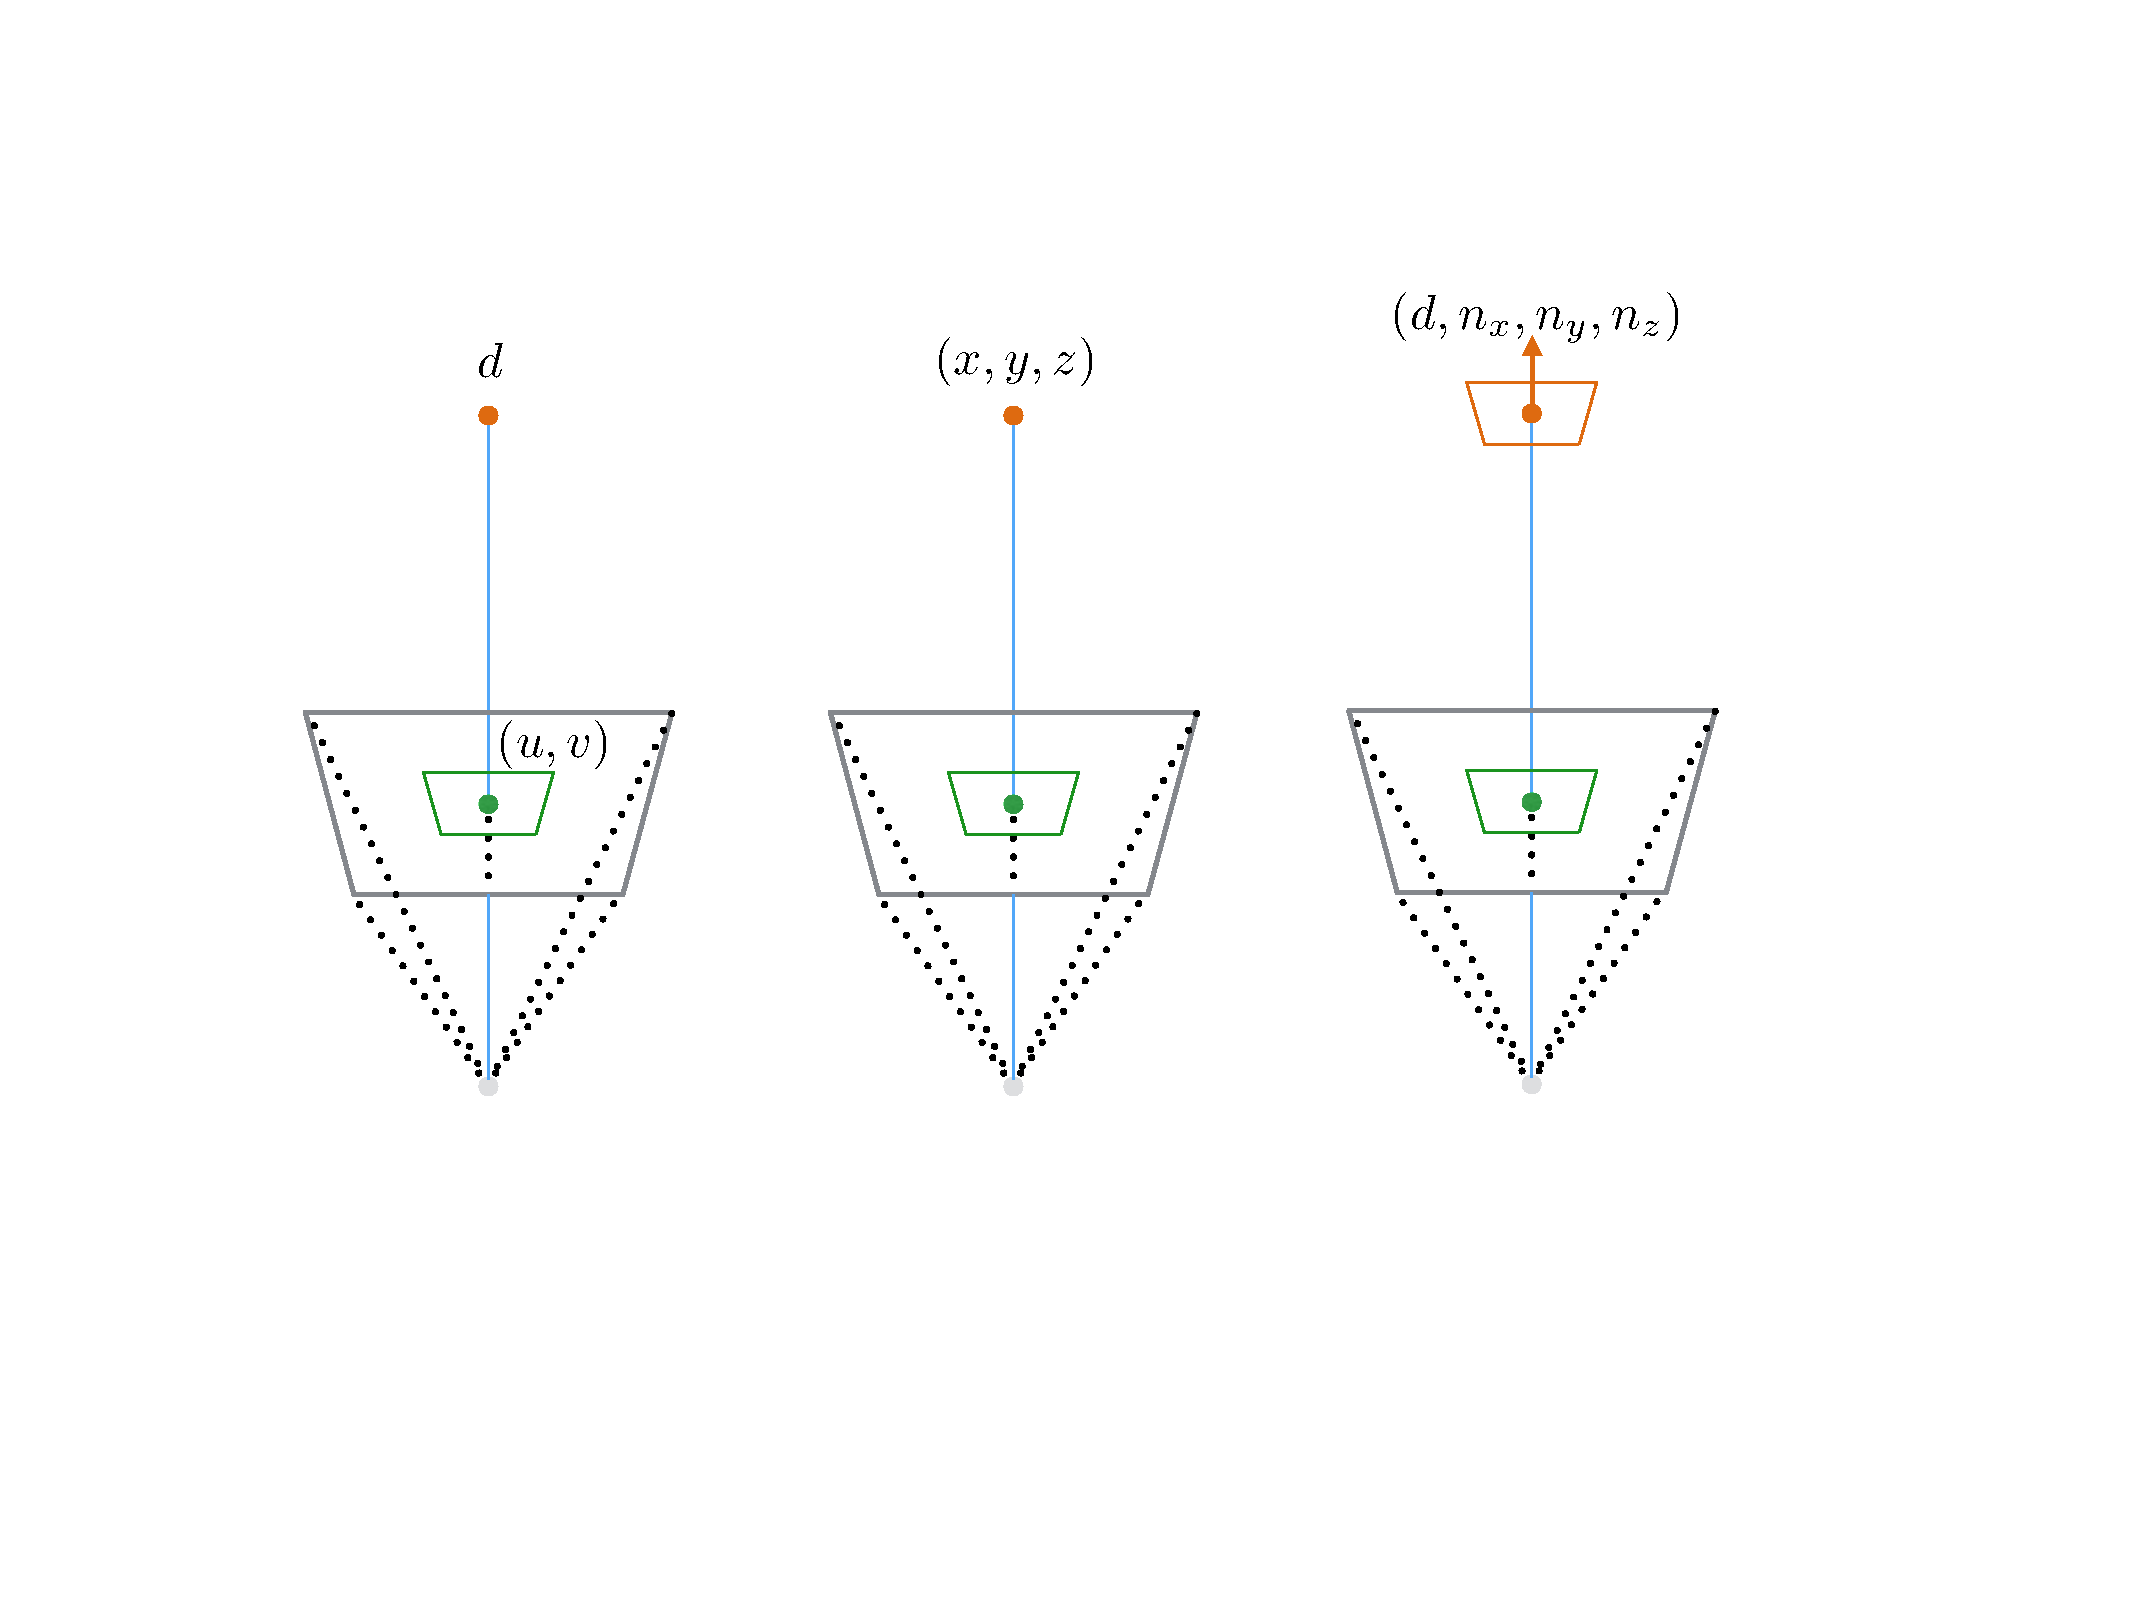
\includegraphics[width=0.8\textwidth]{model/tex_rep}
\caption{scelement and segment representation}
\end{figure}

\subsubsection{Scelement property}
Texture is one of the most important cues for many computer vision algorithms. It is generally divided into two categories, namely \textit{tactile} and \textit{visual} textures. Tactile textures refer to the immediate tangible feel of a surface whereas visual textures refer to the visual impression that textures produce to human observer, which are related to local spatial variations of simple stimuli like colour, orientation and intensity in an image. We focus only on visual textures as it's the most widely used ones in the stereo vision research, thus the term `texture' thereafter is exclusively referred to `visual texture' unless mentioned otherwise.

Although texture is an important component in computer vision, there is no precise definition of the notion texture. The main reason is that natural textures often exhibit different yet contradicting properties, such as regularity versus randomness, uniformity versus distortion, which can hardly be described in a unified manner. Haralick considers a texture as an ``organized area phenomenon'' which can be decomposed into `primitives' having specific spatial distributions~\cite{haralick1979statistical}. This definition, also known as structural approach, comes directly from human visual experience of texture. These primitives are organized in a particular spatial structure indicating certain underlying palcement rules. Alternatively, as Cross and Jain suggested, a texture is ``a stochastic, possibly periodic, two-dimensional image field''~\cite{cross1983markov}, which is also known as \textit{stochastic approach}.

% For s regular textures, there are two basic dimensions on which it may be described. The first dimension is for describing the primitives out of which the texture is composed, and the second dimension is for the description of the spatial dependence or interaction between the primitives of an image texture. The first property is concerned with tonal primitives and local properties, and the second dimension is concerned with the spatial organization of the tonal primitives.

There are various properties that make the texture distinguishable: scale/size/granularity, orientation, homogeneity, randomness, and etc. However, due to the diverse and complexity of natural textures, it's a challenging task to map from these semantic meanings to the precise properties of a synthetic texture. The stereo vision community often take a simplified approach, classifying them into two categories: regular and stochastic ones by their degree of randomness. A regular texture is formed by regular tiling of easily identifiable elements (texels) organized into strong periodic patterns. A stochastic texture exhibits less noticeable elements and display rather random patterns. Most of the real world texture are mixtures of these two categories.

Most texture synthetic research has focused on data-driven or statistical approaches. For the data-driven approach, the generated texture is not general enough whereas it's not intuitive enough for the statistical approach. Thus we turn to an approach that is more tailored to the stereo vision problem. Based on the observations from practical tests, stereo algorithms work well under the condition of non-uniform texture, even for textures caused by shadow. This is theoretically plausible as stereo vision tries to find the correspondence based on the `distinctiveness' of the texture. Therefore, as long as the surface is covered by distinct texture, it doesn't matter what the basic texture element is. Thus the most significant attributes of the texture is coverage, \ie the percent of the surface that is covered, and it's the focus of this thesis.

% Texture is formally defined as a set of texture element or \textit{texels} occuring in some regular, or repeated, or random pattern. Texture gives us information about the \textit{spatial arrangement} of the colours or intensities in an image. However, it is something that is easy to recognize, but hard to define. 

% Here we only consider visual textures, which is the result of shape and reflection. Therefore, a surface with varying reflectance property can produces a textured surface, a flat surface with fixed reflectance property under different illuminations can also achieve textured effect. Even very weak texture can be a strong cue to object reconstruction as manifested by the Middlebury `Dino' dataset.

\subsection{Intensity variation}
When light strikes a surface, it may be absorbed, transmitted, or scattered; usually, a combination of these effects occur. It is common to assume that all effects are local and can be explained with a macroscopic model with no emission, which is called a \textbf{local interaction model}. This is a reasonable model for surfaces that are common in vision. In this model:
\begin{itemize}
\item the radiance leaving a point on a surface is due only to radiance arriving at this point;
\item we assume that all light leaving a surface at a given wavelength is due to light arriving at that wavelength;
\item we assume that the surfaces do not generate light internally and treat sources separately.
\end{itemize}

In this section, we only discuss the intensity that are caused by reflection instead of refraction and transmission, which will briefly touched upon later.

The relation between the incoming illumination and reflected light is model using the \textit{bidirectional reflectance distribution function}, usually abbreviated BRDF. The BRDF is define as

\begin{figure}[h]
\centering
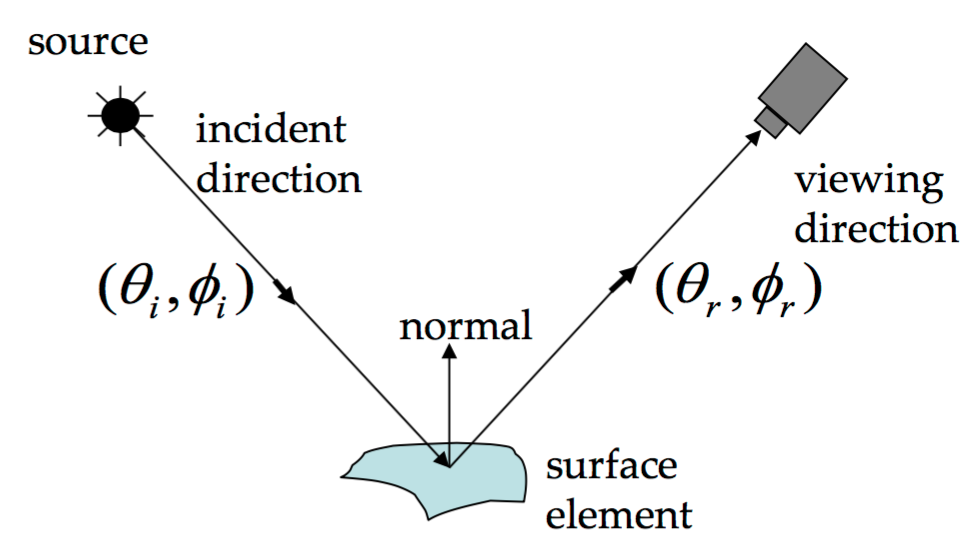
\includegraphics[width=0.5\textwidth]{model/brdf}
\caption{Surface reflection, image courtesy of Srinivasa Narasimhan}
\end{figure}

$\mathbf{E^{surface}(\theta_i, \phi_i)}$: irradiance at surface in direction $(\theta_i, \phi_i)$.

$\mathbf{L^{surface}(\theta_r, \phi_r)}$: irradiance at surface in direction $(\theta_r, \phi_r)$.

\textbf{Definition (BRDF)} the ratio of the radiance of the outgoing direction to the incident irradiance, \ie $f(\theta_i, \phi_i, \theta_r, \phi_r)=\frac{E^{surface}(\theta_i, \phi_i)}{L^{surface}(\theta_r, \phi_r)}$.

\begin{figure}[h]
\centering
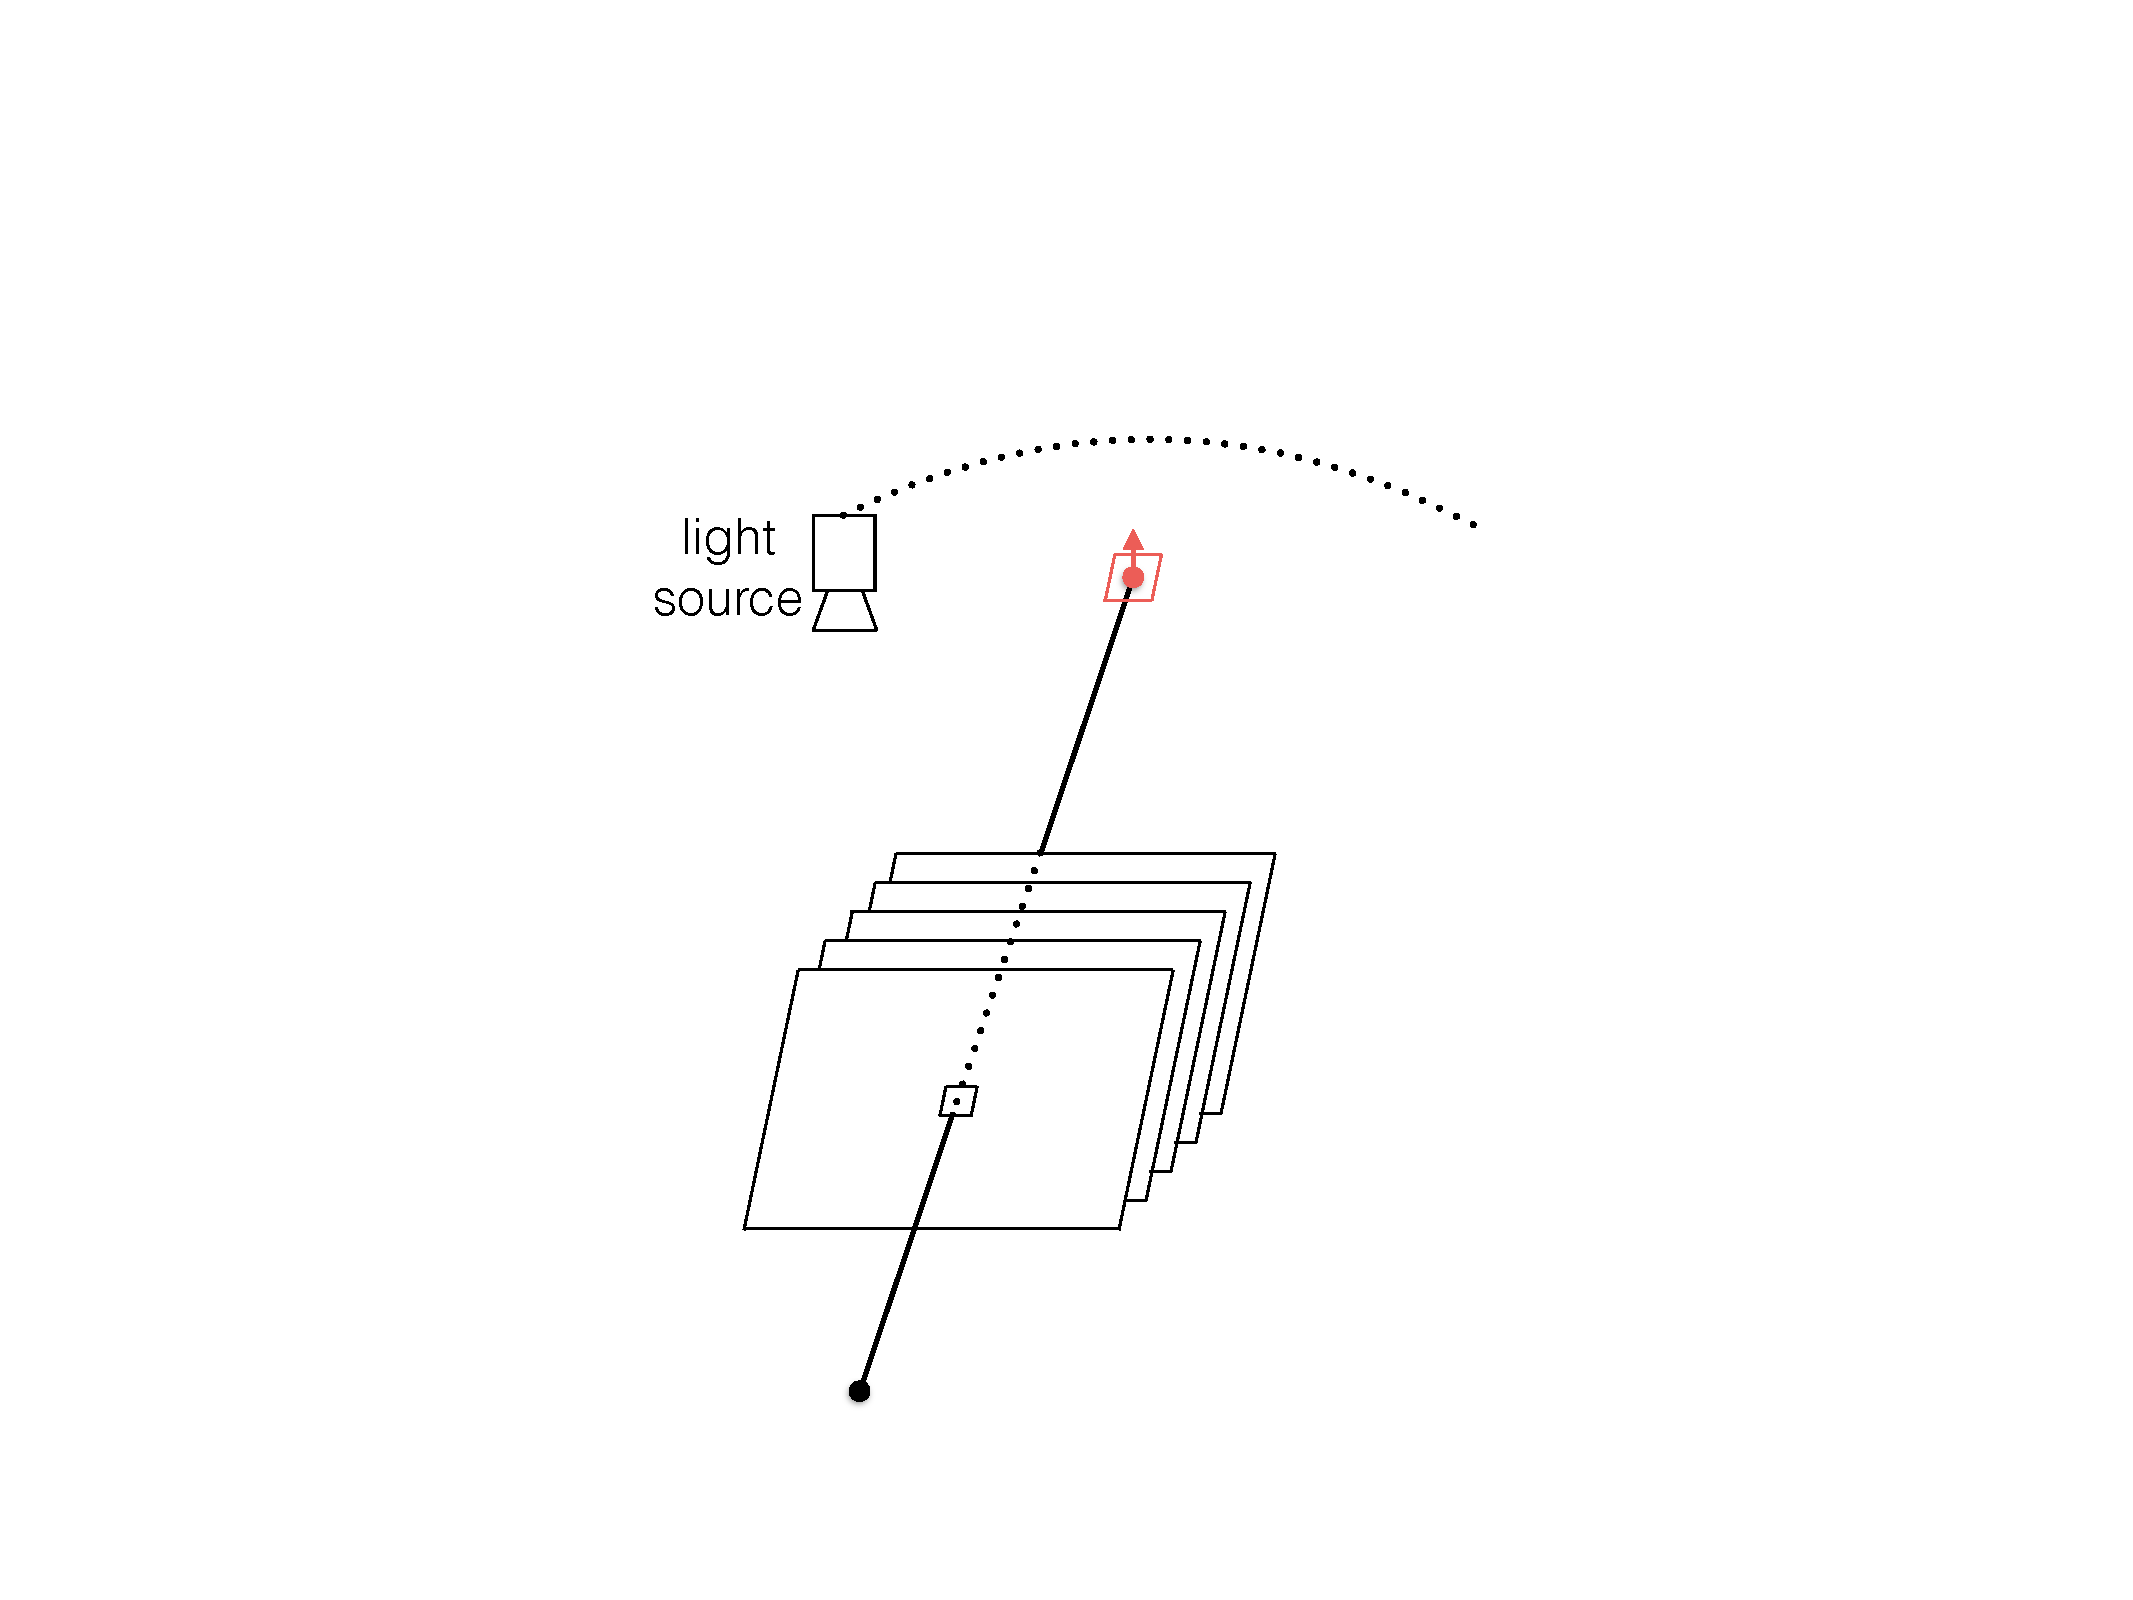
\includegraphics[width=0.6\textwidth]{model/int_rep}
\caption{scelement and segment representation}
\end{figure}

\subsubsection{Diffuse Albedo}
Surface lightness or albedo is the proportion of incident light that is reflected by the surface. It should be noted that albedo is not an intrinsic property of a surface. Instead, for any surface, the albedo depends on the spectral and angular distributions of the incident light. 

The reflectance of light is dependent on the spectrum of the light, which means that the reflectance of the light is dependent on the light frequency, see Figure~\ref{fig:alb_freq}. We consider the reflectance across all spectrum, meaning only intensity albedo is considered.

\begin{figure}[h]
\centering
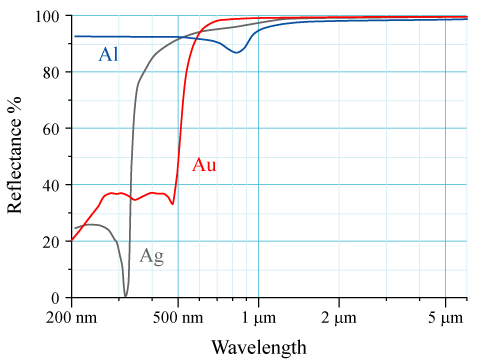
\includegraphics[width=0.5\textwidth]{model/reflectance_frequency}
\label{fig:alb_freq}
\caption{Spectral reflectance curves for aluminium (Al), silver (Ag), and gold (Au) metal mirrors at normal incidence.}
\end{figure}

The reflectance of light also depends on the incident direction. Specifically, light that lands on a surface at a grazing angle will be much more likely to reflect, see Figure~\ref{fig:alb_ang}. We take into account the Fresnel effect in the synthetic stage, thus we consider the albedo with small incident angle.

\begin{figure}[h]
\centering
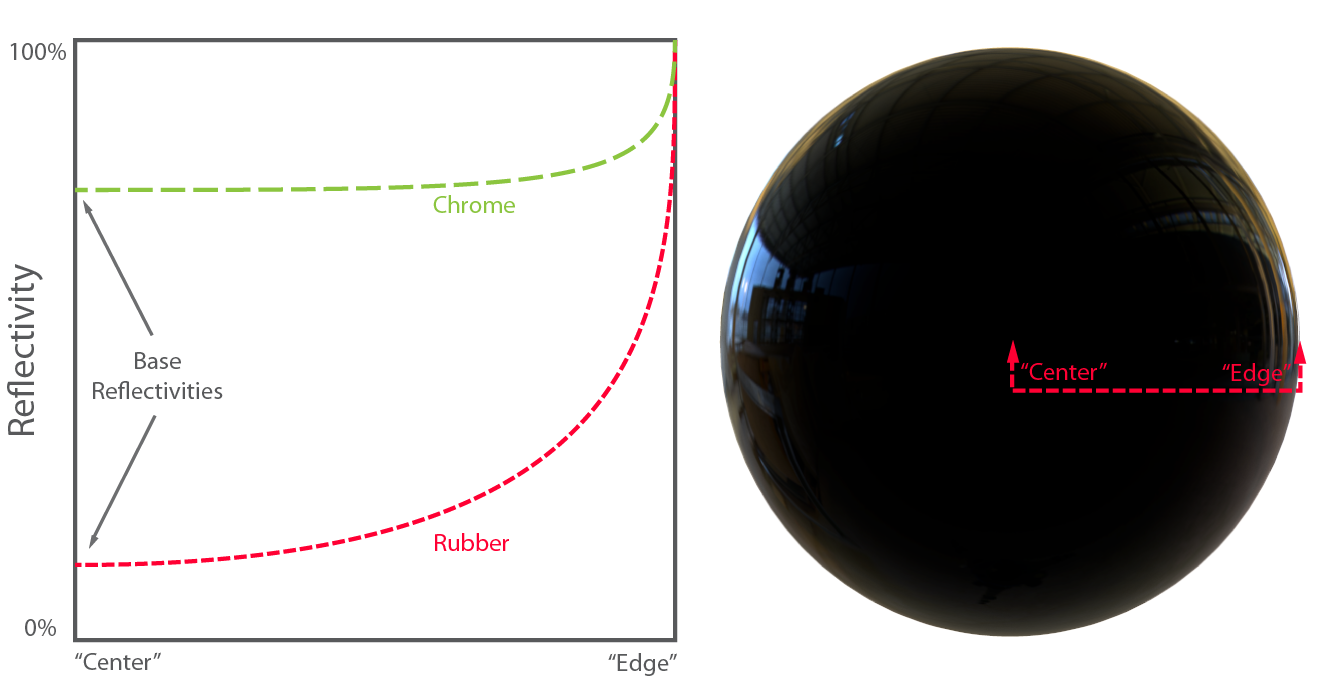
\includegraphics[width=0.5\textwidth]{model/reflectance_angle}
\label{fig:alb_ang}
% \caption{Spectral reflectance curves for aluminium (Al), silver (Ag), and gold (Au) metal mirrors at normal incidence.}
\end{figure}

It ranges from `black' to `white' in the grey scale axis. Colour is a superset intensity, which takes account into the spectral composition of light. Both terms depend on illumination, surface normal, surface reflectance, and viewing direction.

In order to understand the contributing factor of pixel intensity/colour, we need a in-depth understanding of reflection, \ie how light is reflected off of a surface patch, and the relation between incident light and intensity value.

\subsubsection{Specular}
The specular surface reflects light in almost a single direction when the microscopic surface irregularities is small compared to light wavelength, and no subsurface scattering present~\cite{nayar1989surface}. Unlike diffuse reflections, which we experience the lightness and colour of an object, specular reflections carry information about the structure, intensity, and spectral content of the illumination field. In other word, specular reflections are simply images of the environment, or the illumination field, distorted by the geometry of the reflecting surface. See Figure~\ref{fig:lake_spec}, the image no long reflect the original colour of the surface (red), instead it shows a distorted image of the environment. A purely specular surface is a mirror. Purely specular surfaces are rare in nature. Most natural materials exhibit a mix of specular and diffuse reflection. Variations in microscopic surface geometry can cause specular reflections to be scattered, blurring the image of the environment in an amount proportional to surface roughness.

\begin{figure}[h]
\centering
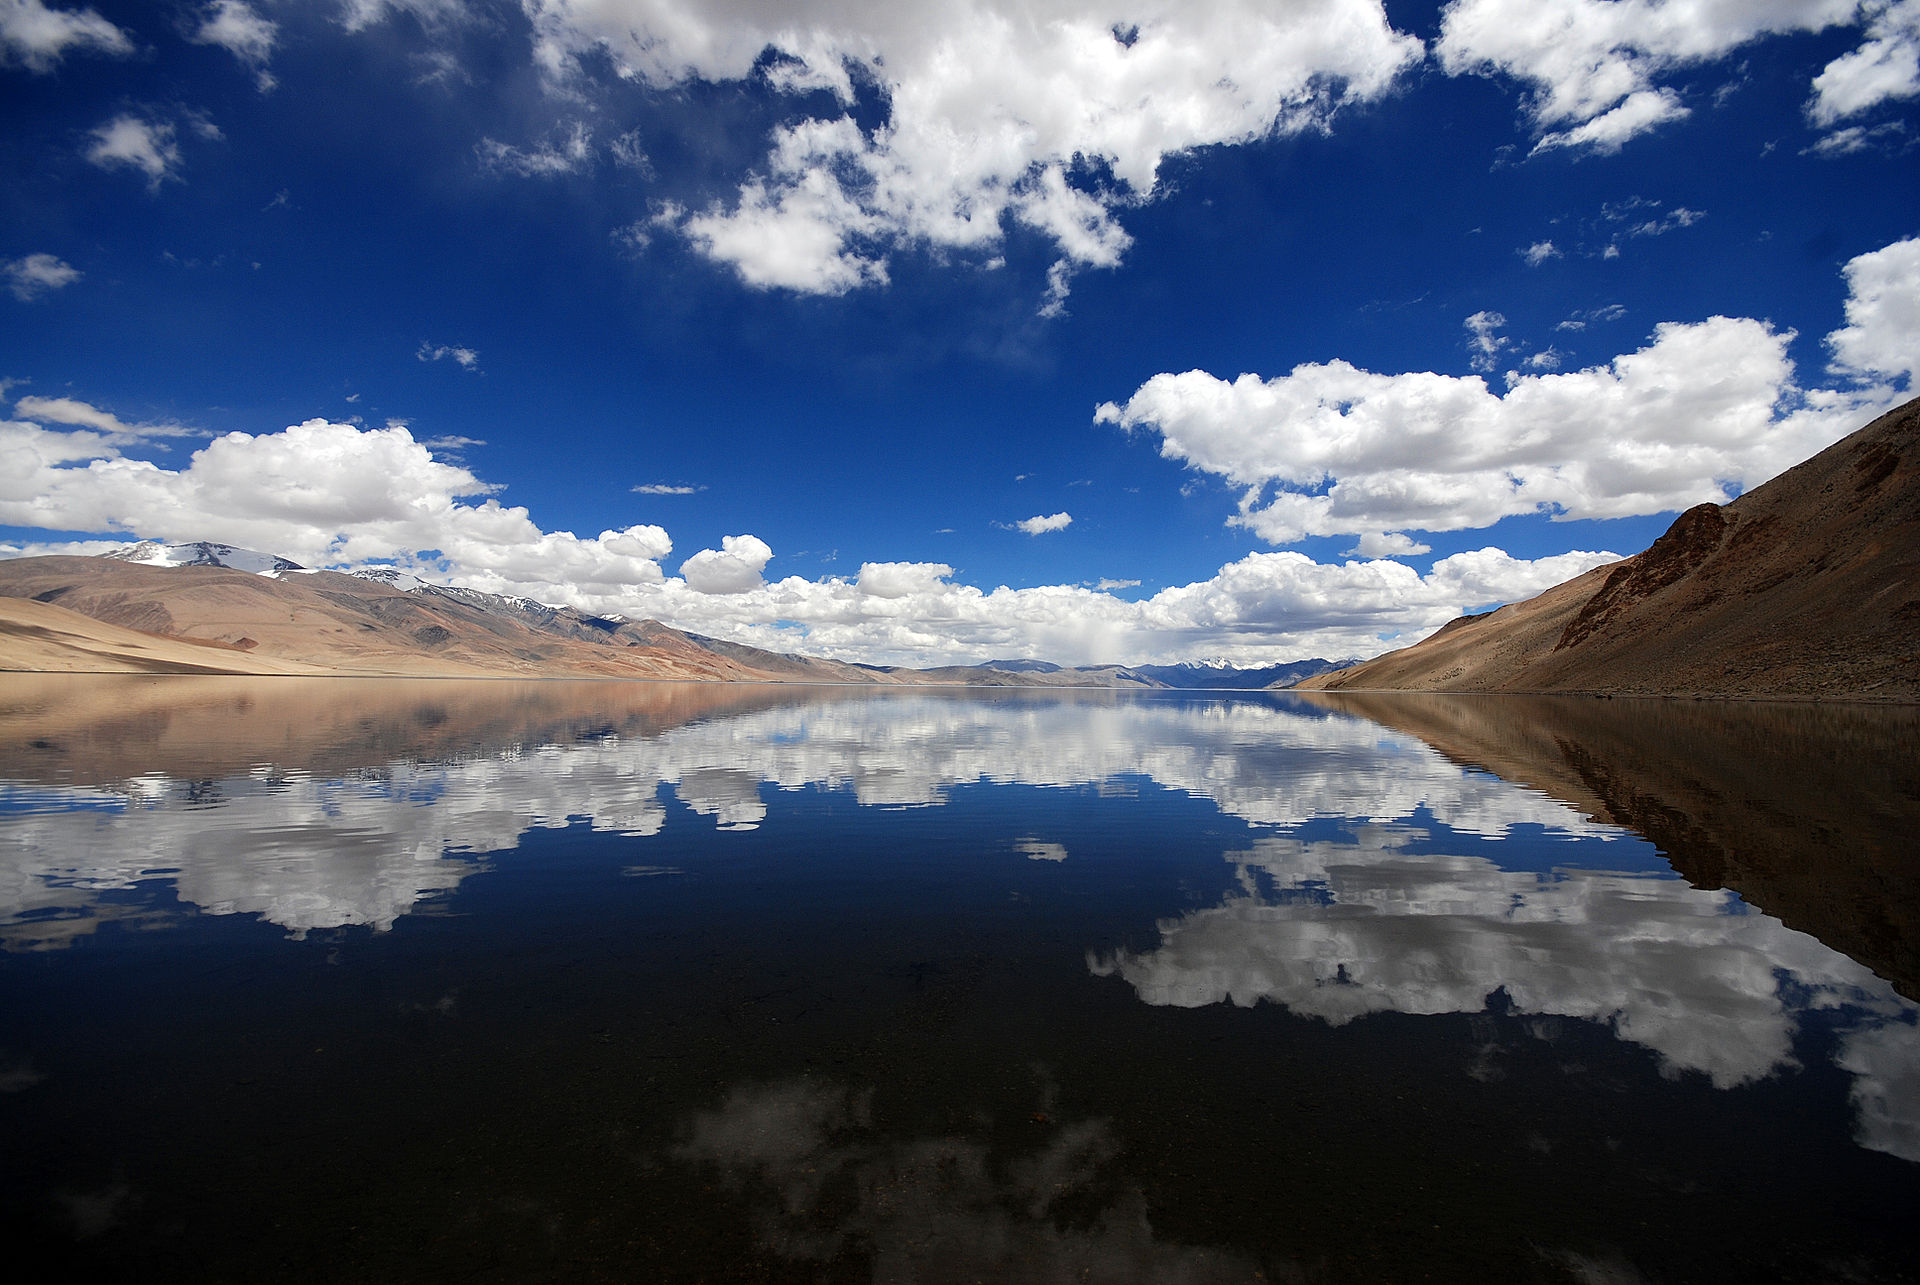
\includegraphics[width=0.5\textwidth]{model/lake_spec}
\label{fig:lake_spec}
\end{figure}

Another observation is that from the image changes as the viewer changes. This can be derived directly from specular reflection, which make stereo correspondence searching extremely challenging.

\subsubsection{Roughness}
The way in which light is reflected by a surface is dependent on, among other factors, the microscopic shape characteristics of the surface. A smooth surface may reflect incident light in a single direction, while a rough surface may scatter the light in various directions. We need prior knowledge of the microscopic surface irregularities, or a model of the surface to determine the reflection of incident light.

The possible surface models are divided into 2 categories: surface with exactly known profiles and surfaces with random irregularities. An exact profile may be determined by measuring the height at each point on the surface by means of a sensor such as the stylus profilometer. This method is cumbersome and impractical. Hence, it’s more reasonable to model the surface as a random process, where it is described by a statistical distribution of either its height above a certain mean level, or its slope w.r.t its mean (macroscopic) slope. The section only discusses these second statistical approach.

% \textbf{Height Distribution Model} The height coordinate of the surface is expressed as random function of the coordinates $x$ and $y$.

% \begin{figure}[h]
% \centering
% \includegraphics[width=0.5\textwidth]{model/surface_representation_1}
% \caption{Surface height distribution model}
% \end{figure}

% The shape of the surface is determined by the probability distribution of $h$. For instance, let $h$ be normally distributed, with mean value $\bar{h}=0$ and standard deviation $\sigma_h$. Then, the distribution of $h$ is given by:

% $$
% p_h(h)=\frac{1}{\sqrt{2\pi}\sigma_h}e^{-\frac{h^2}{2\sigma_h^2}}
% $$

% The $\sigma_h$ is the root-mean-square of $h$ and represents the roughness of the surface. The surface is not uniquely described by the distribution of $h$, as it does not tell us anything about the distance between the hills and valleys of the surface.

% The surfaces below have the same height distribution function, i.e., the same mean value and standard deviation. However, they don't resemble each other in appearance.

% \begin{figure}[h]
% \centering
% \includegraphics[width=8cm]{model/same_mean_sd}
% \caption{Surface height distribution model}
% \end{figure}

% An autocorrelation coefficient $C(\tau)$ is introduced, that determines the correlation (or lack of independence) between the random values assumed by the height $h$ at two surface points $(x_1, y_1)$ and $(x_2, y_2)$, separated by a distance $\tau$. The autocorrelation coefficient can be:

% $$
% C(\tau)=e^{-\frac{\tau^2}{T^2}}
% $$

% where $T$ is the *correlation distance*. Therefore, the above surfaces have small and large correlation distances respectively.

\textbf{Slope Distribution Model} We can also think of a surface as a collection of planar micro-facets.

\begin{figure}[h]
\centering
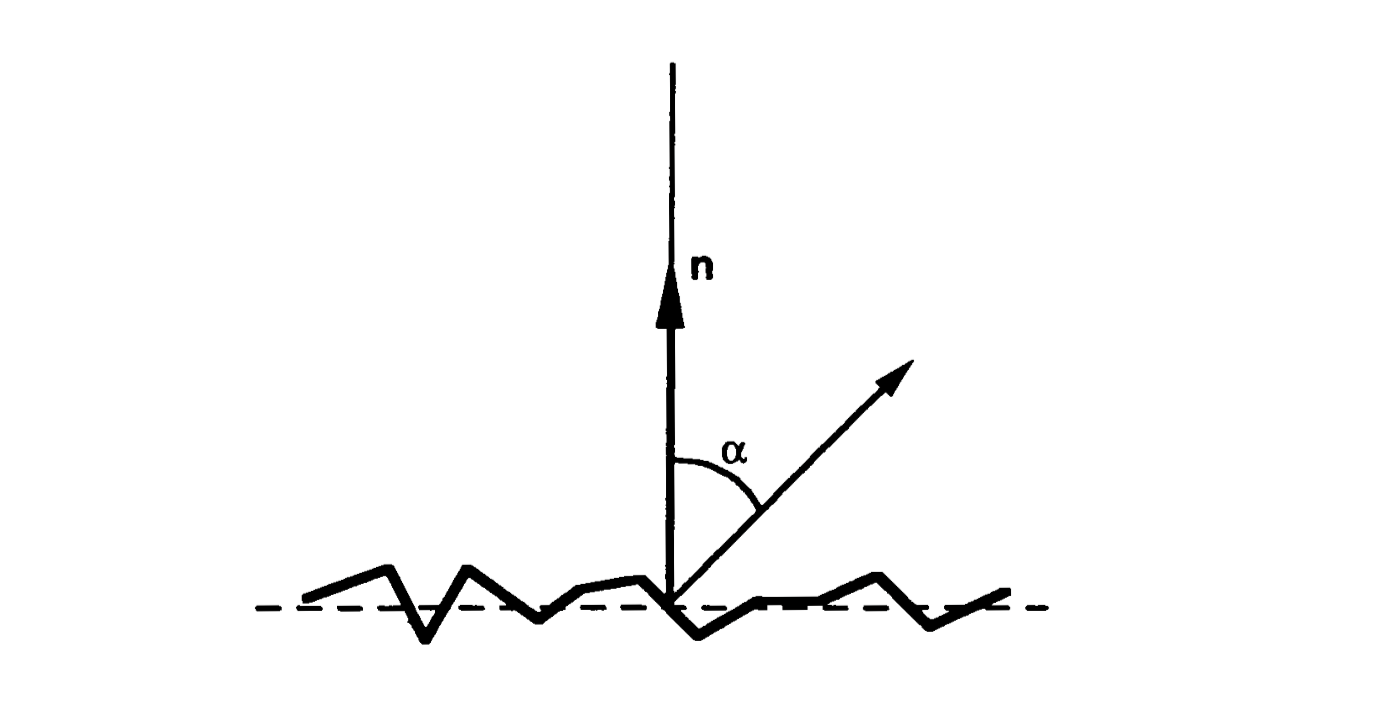
\includegraphics[width=0.7\textwidth]{model/surface_representation_2}
\caption{Surface Slope Distribution Model}
\end{figure}

A large set of micro-facets constitutes an infinitesimal surface patch that has a mean surface orientation $\vec{n}$. Each micro-facet has its own orientation, which may deviate from the mean surface orientation by an angle $\alpha$. 

We will use the parameter $\alpha$ to represent the slope of individual facets. Surfaces can be modeled by a statistical distribution of the micro-facet slopes. If the surface is isotropic, the probability distribution of the micro-facet slopes can be assumed to be rotationally symmetric w.r.t the mean surface normal $\vec{n}$.  Therefore, facet slopes can be described by a one-dimensional probability distribution function. For instance, the surface may be modeled by assuming a normal distribution for the facet slope $\alpha$, with mean value $\bar{\alpha}=0$ and standard deviation $\sigma_\alpha$:

$$
p_\alpha(\alpha)=\frac{1}{\sqrt{2\pi}\sigma_\alpha}e^{-\frac{\alpha^2}{2\sigma_\alpha^2}}
$$

The surface model is determined by a single parameter $\sigma_\alpha$, and larger $\sigma_\alpha$ can be used to model rougher surfaces. While autocorrelation coefficient is important, the concept of slope correlation is more difficult to interpret and is not that useful in the generation of surface, which results in a weaker model compared to the height model. However, slope distribution model is popular in the analysis of surface reflection, as the scattering of light rays is dependent on the local slope of the surface and not the local height of the surface.

% surface roughness will affect the fresnel and specularity

% \subsubsection{Sub-surface Scattering}
% Sub-surface scattering can also cause diffuse reflection.

\subsubsection{Concavity}
Concavity can cause self-shadow or inter-reflection effect, which can severely impede the accuracy of intensity based algorithms. Since concavity is not shown in the silhouette image, methods that utilize silhouette information may also fail to reconstruct concavities. Concavity is measured by \textit{surface curvature}.

\subsubsection{Silhouette}

% \subsection{Inputs}
% \subsection{Outputs}
% \subsubsection{Volumetric Grid}
% \subsubsection{Point Cloud}
% \subsubsection{Surface Mesh}
% \subsubsection{Depth/Height Map}
% \subsubsection{Normal Map}

\section{Expression}
\label{sec:3DRecon_Exp}

\subsection{MVS}

\subsection{PS}

\subsection{SL}
